\chapter{Analyse}\label{k_analyse}

% Beschreibung des Aufbaus
\section{Versuchsaufbau}
\begin{figure}[h] \centering
	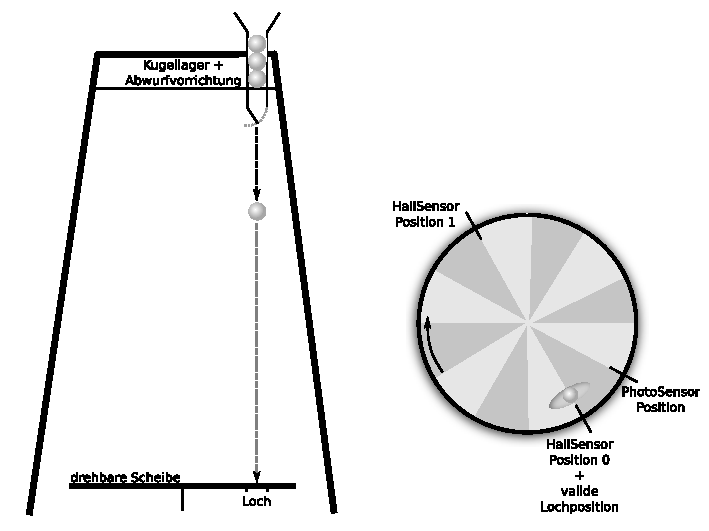
\includegraphics[width=\textwidth]{images/aufbau.pdf}
	\caption{schmatischer Versuchsaufbau - v.\,l.\,n.\,r. Seitenansicht Gesamtaufbau, Drehbare Scheibe}
	\label{img:versuchsaufbau}
\end{figure}

\begin{figure}[h] \centering
\begin{tabular}{lc} 
	\textbf{Eigenschaft} 	& \textbf{Beschreibung}	\\
	\toprule
	\multicolumn{2}{c}{Tisch}\\ 
	\midrule
	Abwürfhöhe 	& 750\,mm \\
	\#Schwarzer Felder 	& 6 \\
	\#Weiße Felder 	& 6 \\
	Lochlänge innen 	& 55\,mm \\
	\midrule 
	\multicolumn{2}{c}{Kugel}\\ 
	\midrule
	Masse 	& 8.5\,g \\
	Durchmesser 	& 12\,mm \\
	\bottomrule
\end{tabular}
\end{figure}

Der Hallsensor zeigt zwei mal pro Umdrehung exakt die Position der Scheibe an.
Dies geschieht, wenn das Loch an \texttt{HallSensorPosition1} und \texttt{HallSensorPosition0} ist (siehe Abb. \ref{img:versuchsaufbau}), wobei zweiteres der Position entspricht, an welcher die Kugel durch das Loch fallen muss.
An den Positionen wechselt die Ausgabe der Sensoren auf den entsprechenden Wert, daher 1 bzw. 0.

Der Photosensor gibt abhängig davon, ob er eine helle oder dunkle Fläche vor sich hat eine 1 oder 0 aus.
Da die Felder auf der Unterseite der Scheibe gleichmäßig verteilt sind (siehe Abb. \ref{img:versuchsaufbau}), kann er nicht zur Positionsbestimmung, dafür für die Bestimmung der Drehgeschwindigkeit verwendet werden.

Die Sensorwerte einer Scheibenumdrehung sind in Abb. \ref{img:sensorwerte} geplottet.

\begin{figure}[h] \centering
	\includegraphics[width=\textwidth]{images/generated/sensor_messwerte1.pdf}
	\caption{Sensorzyklus einer Scheibenumdrehung}
	\label{img:sensorwerte}
\end{figure}

\section{Fallzeit der Kugel}
Um die Fallzeit einer Kugel zu berechnen wird die Formel für den freien Fall im homogenen Feld
\begin{align}
	t(h) = \sqrt{\frac{2h}{g}}
\end{align}
verwendet.
Setzt die oben beschriebenen, am Versuchsaufbau gemessenen, Messwerte ein

\begin{align}
t(h) &= \sqrt{\frac{2 * 0.75m}{9.81\,\nicefrac{m}{s^2}}} \\
	 &= 0.391\,s \\
	 &= 391\,ms
\end{align}
so kommt man auf eine Fallzeit von 391\,ms für eine Kugel.



% Approximationskurve
\begin{figure}[hb] \centering
	\includegraphics[width=\textwidth]{images/generated/Data4.pdf}
	\caption{Drehgeschwindigkeit über der Zeit approximiert mit der Funktion: \newline $u(t) = 150.9575 - 1.5678\cdot t + 0.0036 \cdot t^2$}
\end{figure}

